\documentclass[dvipdfmx]{jsarticle}

\usepackage[version=3]{mhchem}
\usepackage{amsmath}
\usepackage[siunitx]{circuitikz}
\usepackage{graphicx}
\usepackage{here}

\setlength\parindent{0pt}

\begin{document}
\title{情報通信工学レポート}
\author{工学部電子情報工学科3年 03190449  堀 紡希}
\date{\ 9月28日}
\maketitle

\section{レポート課題1}


\begin{figure}[H]
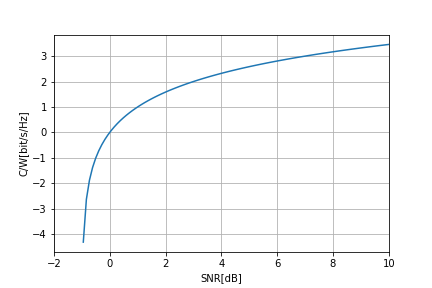
\includegraphics[scale = 0.8]{1.png}
\caption{信号対雑音電力比と周波数利用効率の関係}
\end{figure}

\section{レポート課題2}


\begin{figure}[H]
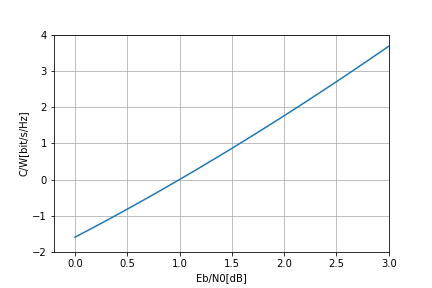
\includegraphics[scale = 0.8]{2.png}
\caption{デジタル伝送路における信号対雑音電力比と周波数利用効率の関係}
\end{figure}

$E_{b} = \frac{P}{C}$を代入して、

\[ \frac{E_{b}}{N_{0}} = (2^{\frac{C}{W}}-1)\times \frac{W}{C}\]

$\frac{C}{W} \to 0$の時、$\frac{C}{W} = x$とおくと、ロピタルの定理より、
\begin{align*}
\lim_{\frac{C}{W} \to 0} \frac{E_{b}}{N_{0}} &= \lim_{x \to 0} \frac{2^{x}-1}{x} \\
&= \lim_{x \to 0} \frac{\log{2}\times 2^{x}}{1} \\
&= \log{2} \\
&= -1.59[dB]
\end{align*}
となり、シャノン限界を確認できる。

\section{レポート課題3}
$f \neq 2$の時
\begin{align*}
\int _{0} ^{1} \cos{4\pi t}\cos{2\pi ft} &= \int _{0}^{1} \frac{1}{2}(\cos{(4\pi t + 2\pi ft)}+\cos{(4\pi t - 2\pi ft)})\\
&= \frac{1}{2} ([\frac{\sin{4\pi t + 2\pi ft}}{4\pi + 2\pi f}]^{1} _{0} + [\frac{\sin{4\pi t - 2\pi ft}}{4\pi - 2\pi f}]^{1} _{0}) \\
&= (\frac{1}{4\pi + 2\pi f} + \frac{1}{4\pi - 2\pi f})\sin (2\pi f)
\end{align*}

よって直交する、すなわちこの式が0になる$f$で最小の$f$は
\[f = \frac{1}{2}\]

\end{document}